\documentclass[a4paper]{article}
\usepackage{booktabs}
\usepackage{fancyhdr}
\usepackage[english]{babel}
\usepackage[utf8]{inputenc}
\usepackage{amsmath}
\usepackage{hyperref}
\usepackage{graphicx}
\usepackage[colorinlistoftodos]{todonotes}
\usepackage{float}
\usepackage{caption} \captionsetup[table]{skip=5pt}

\usepackage{multirow}
\usepackage{url}
\usepackage{subcaption}

\begin{document}

\title{\textbf{\huge Optimising similarity search between images}\  \\  \textit{Semester Project}\vspace{3 cm}}

\author{Author:\\ Guillaume RAILLE \vspace{1 cm}\\ Supervisors: \\ Prof. Karl ABERER \\ Rémi LEBRET \\ Hamza HARKOUS  \vspace{3 cm}}



\date{Winter 2017}


\begin{figure}
\centering

\includegraphics[width=0.7\textwidth]{epfl}
\end{figure}
\renewcommand{\headrulewidth}{1pt}
\fancyhead[L]{Semester Project}
\fancyhead[R]{Optimising Similarity Search}

\maketitle
\pagestyle{fancy}

\newpage
\section*{Introduction}
	\subsection*{Purpose of this project}
	This project takes an experimental approach to implement, assess and compare different solutions to efficiently detect similarities between images. It is based on several state-of-the-art techniques and methodology that are still actively growing and being developed today such as Convolutional Neural Network and transfer learning. The way to address the issue of detecting similarities between images at large scale was largely influenced by this paper \cite{large-scale-search}. It can be considered as a solid starting point for this project as it helped us define an efficient pipeline and evaluation methodology.
	
	\subsection*{Some definitions}
		\subsubsection*{Convolutional Neural Network (CNN)}
		
		As we introduced just above, Convolutional Neural Network are at the essence of this project and understanding the idea behind it was also part of the project. In our case we consider a Convolutional Neural Network that takes as input an image, perform multiples operation and convolution on it and gives as output a fully connected layer (FC) that is just a one dimension vector with each value of this vector being a weight that represent the vote of a given image to be part of a given class. The different values of the masks (in the the convolutional layers) and the voting weights are learn through back propagation (gradient descent). There are nowadays many implementations of CNN. In this project, we focused on a CNN called ResNet which was developed at microsoft for the COCO 2015 competition \cite{resnet}. ResNet stands for Residual network, they were the first to introduce shortcut connections between layers to improve the performance of their CNN. More specifically we used throughout the project their 18-layers ResNet implementation.
		
		\subsubsection*{Transfer learning}
		
		The problem with CNN is that before it is trained and its voting weights and values are learned from the data, it is absolutely useless. Unfortunately, before becoming very performant, CNN usually needs to be trained on a lot of data and it takes a very long time. Transfer learning solves this problem by using a pre-trained CNN (on an unrelated dataset) to solve our specific classification problem. There is basically two ways to perform transfer learning: Finetuning or Fixed Feature extractor. The first one consist in using pretrained weights instead of random initialisation, the second one consist in fixing the weights for all the network except the Fully Connected layer. The latter is much faster and our project pipeline is based on this concept.

		\subsubsection*{Hardware and Setup}
		The aim of best efficiency to perform large scale similarity between image detection is obviously highly dependent on the hardware used to perform the search in the first place. In our case, we had the opportunity to compare on a server the difference between method using GPU and CPU. During the project we used a Nvidia Titan X to perform the computation on GPU, and an Intel(R) Xeon(R) CPU E5-2620 v3 with 24 cores for computation on CPU. To easily handle GPU computation and switch between CPU/GPU memory, we used the open-source Pytorch library.
		
\section{Pipeline}

To evaluate efficiently the different method to detect similarities, we followed a pipeline similar for each method tested. As previously mentioned, this pipeline is highly inspired from this paper \cite{large-scale-search}. This pipeline is composed of three steps before assessment or evaluation of the results. First we perform a Feature extraction on each image using a pretrained CNN, then we perform a PCA dimensionality reduction to improve the speed and performance of the computations, finally we apply the k-NN (nearest neighbour) method we want to test on the PCA reduced extracted features.


\subsection{Feature Extraction}

The Feature Extraction step of our pipeline is very similar to what we described in transfer learning (Fixed Feature extractor). Here as well we used a pretrained CNN (ResNet-18) trained on ImageNet and Places365 (see more in Datasets section) and we fixed their weights. Then we extracted for each images the "features" corresponding to the output of the last convolution layer (just before the fully connected layer). In this specific case we ended up with a one vector with 512D for each images in our dataset. The output of last Layer of our CNN represent the high-level features from our convolutional neural network and describe each corresponding image with this 512 values. We could use this "description" of the images as is and perform directly the third step to find the most similar images inside our dataset but to optimise the process we decided to use PCA following the pipeline from the paper \cite{large-scale-search}.  

\subsection{Dimensionality Reduction (PCA)}

How we realise PCA to reduce the number of feature through SVD.
Led to two datasets that we used through this project (Raw features and PCA features)
The extracted features from each images aggregated in a matrix, we obtained from the first step a (\# of images x 512) dimension matrix. Reducing the dimension using PCA in this case from 512 to 128 helped us to get a great increase in computation time while keeping a good accuracy (see results). To perform PCA on GPU we used the SVD pyTorch function which perform the SVD decomposition. From the SVD decomposition we could compute the dimension reduced matrix (with Û*S) equivalent to the PCA reduction. This dimensionality reduction led to the use of 2 datasets throughout the project:
\begin{itemize}
	\item raw features (corresponding to the raw 512D vector extracted for each image)
	\item PCA features (corresponding to the 128D PCA reduced vector for each image).
\end{itemize}

\subsection{k-NN methods}

The last step of our pipeline was to actually compute similarities between images using the features previously extracted. To do so we used different k-NN methods and we evaluated their performance. We tried some on GPU other on CPU and we even compared with our on implementation of k-NN.

\subsubsection{Bruteforce}

What we call in this project simply "Bruteforce" was our own implementation of a k-NN Bruteforce method. It is a very simple method that simply check all possible neighbour and return the closest one. We made it run on GPU using two already optimised function from PyTorch: "topk" to find the k closest neighbour and "norm" to compute the distance between features vector. We mostly used this approach to produce a "k-NN ground truth" that can be use to compare other approximate method performance. It is also useful to check their computation time performance against this simple bruteforce method.

\subsubsection{Annoy}

	Annoy\footnote{\url{https://github.com/spotify/annoy}} is an approximate Nearest Neighbors library developed in C++ and optimised for memory usage and loading/saving to disk. It was built by Erik Bernhardsson at Spotify during Hack Week and is still currently being used by Spotify. It supports a full Python API that we will be using in this project. The main advantage of this library (beside the fact that it is fast and it is optimised to reduce footprint memory), is that it has the ability to use static files as indexes to compute k-NN. In particular, it makes it possible to pass around indexes as files and map them into memory quickly. Annoy was only developed for CPU and as such we will only use it on our CPU. It is also worth noting that Annoy is an approximate method and we will need to compare it with an exact method (bruteforce) to assess its performance. \\
	
	On a more practical point of view, Annoy uses Random Projection to build up a tree. At every intermediate node in the tree, it divides the space into 2 subspaces using a random hyperplane (hyperplane chosen by sampling two points from the subset and taking the hyperplane equidistant from them). Doing this operation multiple times will generate of forest of trees which represent the index previously mentioned. As such Annoy let us play with 2 parameters:
	
	\begin{itemize}
		\item \textit{n\_trees}: the number of tree we are willing to build. More \textit{n\_trees} implies more build time and more memory usage but also more precision.
		\item \textit{search\_k}: the number of node to inspect when searching for nearest neighbour in the trees. Higher \textit{search\_k} leads to higher precision but increase the search computation time as well.
	\end{itemize}

\subsubsection{NMSLIB}

NMSLIB\footnote{\url{https://github.com/searchivarius/nmslib}} or Non-Metric Space Library (NMSLIB) is an efficient cross-platform similarity search library and a toolkit for evaluation of similarity search methods. It allows searching in generic metric and non-metric spaces. In our case we only focus on the euclidian space. Indeed we use a l2 norm to find similarity between extracted features. This is a good news as NMSLIB claims to have very good performance in the Euclidian domain as well. NMLSIB has been developed and optimised in C++ and also provide a Python API that we use in this project. The library propose many different similarity search methods with different performance in this project we will focus on one of the most promising one they provide: Hierarchical Navigable Small World graphs (also known as HNSW \cite{HNSW}). This approximate approach is fully graph-based, without any need for additional search structures and is able to strongly outperform many previous state-of-the-art vector-only approaches. NMSLIB has been written for CPU and as such we will make or computation on the CPU we have at hand. When using HNSW the only parameter we will be able to tune will be the number of worker (number of threads used by the CPU).

\subsubsection{Faiss}
\begin{itemize}
	\item What is Faiss? \vspace{5pt} \\
	Faiss\footnote{\url{https://github.com/facebookresearch/faiss}} is a library that was originally developed at Facebook AI research. The library was at the beginning a project that led to a published paper \cite{faiss}. At its essence, the project focused on similarity search at "billion scale" by optimizing GPU usage. The library that came out of it (faiss) is by nature optimize for GPU and propose an efficient design for brute-force, approximate and compressed-domain search based on product quantization (Voronoi cells).
	\item How did we use Faiss? \vspace{5pt} \\
	On a more practical point of view the Faiss library is also very efficient to perform similarity search on CPU, but we focused in this project on the GPU performance of it as it is where the library shine. We applied the usual pipeline on Faiss, the only singularity here was that the library offered much more possibilities compared to all the previous one. In order to properly assess the performance of Faiss approximate method, we made several benchmarks playing around with the parameters (mostly nlist representing the number of voronoi cell to split our data on, and nprobe the number out of nlist to check when performing the search). We first did our experiment on a k-NN search with k=2 to get the vector itself and its nearest neighbour then we repeated our analysis with k=6 to get the 5 closest neighbours.
\end{itemize}


\section{Experimental Setup}

Now that we set in the previous part a Pipeline to study and evaluate our different approach to image similarity detection. We will describe here what we use in practice in our experimental approach to the problem.

\subsection{Datasets}
All in all, we used three different dataset in this project for two main purpose: two dataset for feature extraction and one dataset to evaluate the performance of our methods.

\subsubsection{ImageNet and Places365 for feature extraction}
As described in the introduction (c.f. transfer learning) and in the feature extraction of the Pipeline part (c.f. 1.1), it is wise to extract the features directly from a pretrained network. After choosing the CNN we were going to use (ResNet-18) we had several choices regarding on which data it was going to be trained. We chose in this project to study and see the resulting difference between two training datasets:
\begin{itemize}
	\item \textbf{ImageNet\footnote{\url{http://www.image-net.org}}}: ImageNet is a very wide library of labeled images (almost 14.2 millions images) organized according to the WordNet hierarchy (tree of words) in which each nodes represent an average of 500 words. ImageNet is very famous for the challenge they propose (LSVRC) from which many image classification solution and in particular CNN where developed such as the ResNet used during this project. It's important to note that most images from this library are precisely zoomed at one or a few particular object corresponding to the word they are stored at. (see Figure \ref{fig:imagenet-img} for an example)
	\item \textbf{Places365\footnote{\url{http://places2.csail.mit.edu}}}: Places365 is a dataset composed of 1.6 million train images from  365 scene categories. The images are labeled and represented by meta attribute in this case mostly attributes as well as a scene category. In this dataset, the pictures represent each time a whole scene (see Figure \ref{fig:places-img}) and not a precise object as in ImageNet. We will see the influence of it in the last part of this project where we compare the performance of our Pipeline on different subgroup of images.
\end{itemize}

Using transfer learning and pretrained CNN has some advantages and inconvenient that we will mostly see in the last part of this project (Images subgroup analysis). Most of the results obtained in this project and unless specified otherwise will result from features extracted from the ResNet-18 pretrained on the ImageNet dataset.


\subsubsection{MSCoCo for evaluation}

To test the different method and get meaningful results we needed a third independent dataset. This dataset had to be wide as we were willing to perform our evaluation at large scale. This is the reason why we used the COCO\footnote{\url{http://cocodataset.org}} dataset for evaluation. COCO is a large dataset of more than 330'000 images humanly labeled with caption. The images present in this dataset are again more representing a scene rather than a specific object as we can see on Figure \ref{fig:coco-img}. All the results we obtained are coming from the training set 2017 of the COCO challenge which is composed of roughly 118'000 images with 5 humanly made caption each. Another good aspect of using COCO is that it provide an integration with Pytorch and makes it easy to load the images and their corresponding captions through the COCO API.


\begin{figure}
  \begin{subfigure}[b]{0.32\textwidth}
    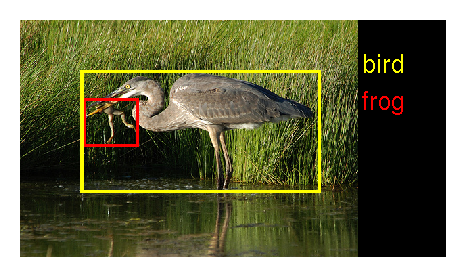
\includegraphics[width=\textwidth, height=3cm]{imagenet-img}
    \caption{ImageNet image}
    \label{fig:imagenet-img}
  \end{subfigure}
  %
  \begin{subfigure}[b]{0.32\textwidth}
    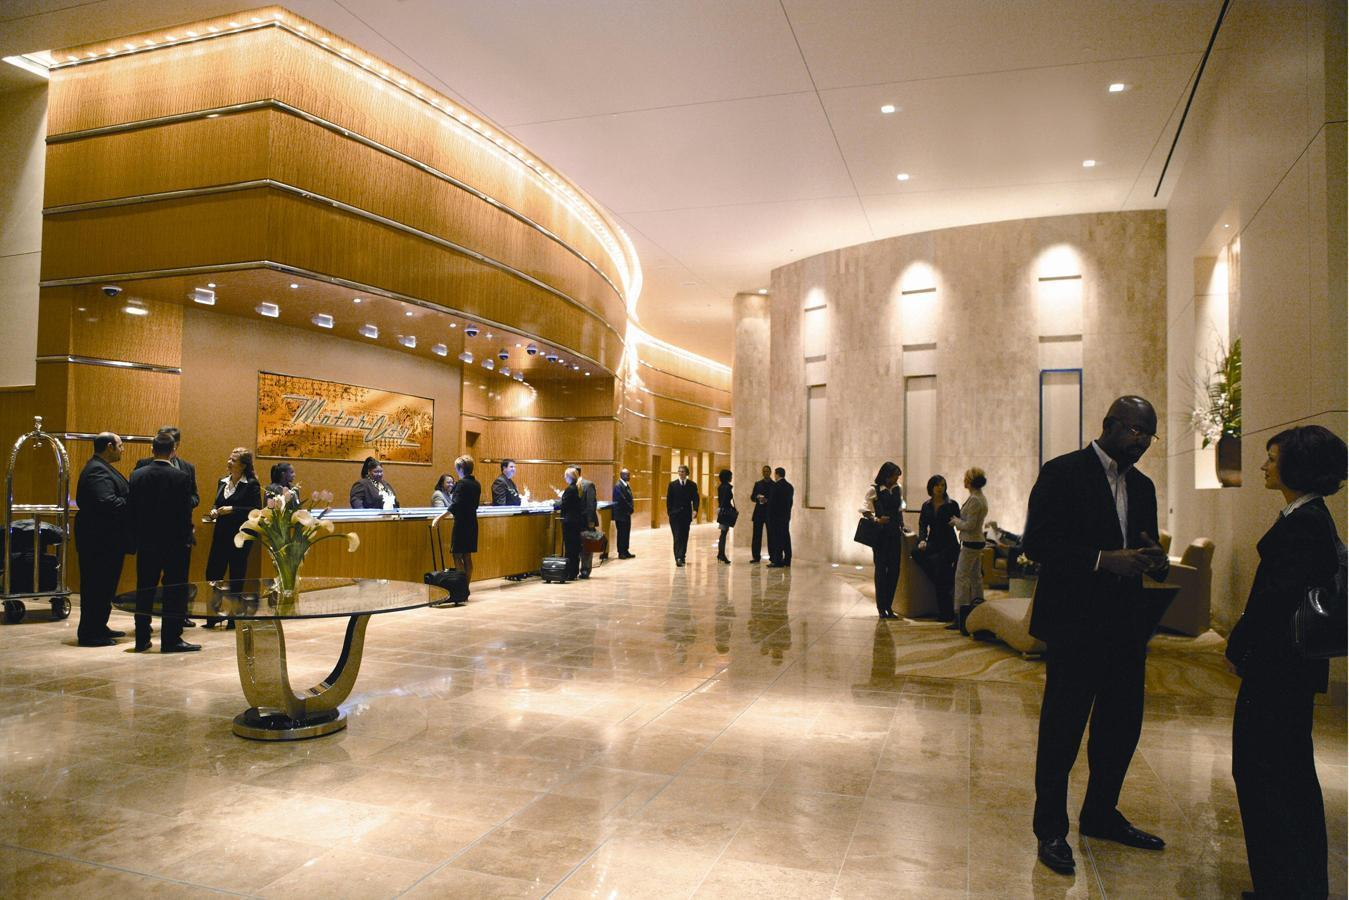
\includegraphics[width=\textwidth, height=3cm]{places-img}
    \caption{Places365 image}
    \label{fig:places-img}
  \end{subfigure}
  %
  \begin{subfigure}[b]{0.32\textwidth}
    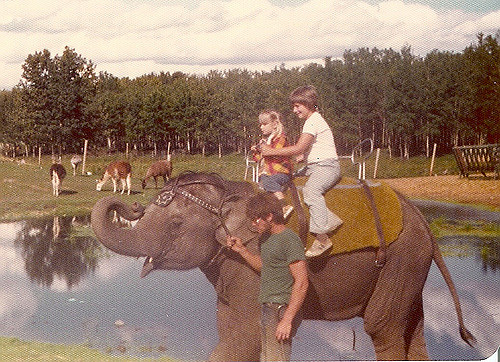
\includegraphics[width=\textwidth, height=3cm]{coco-img}
    \caption{COCO image}
    \label{fig:coco-img}
  \end{subfigure}
\end{figure}

\subsection{Evaluation Technique and Metrics}

After performing the different operation of our pipeline on the datasets, we wanted to evaluate the performance of the different k-NN method and library tried during the process. To do so a measure we constantly used during the evaluation phase was the computation time in second. If the method used some kind of indexing we also computed separately the time of building the index, the time of searching on the index, and the total time. As we are using a several approximate method, it is also interesting to look a the performance of the result for that we use two strategies described below: Similarity in result with the ground truth (brute-force search), and Bleu score. 

	\subsubsection{Compare similarity with brute-force}
		2 kinds of similarity (strict and permissive)
		To compare the similarity between two results from different library we computed their similarity with our basic brute-force results. It is important to note that since the brute-force also use approximation to compute their neighbours (floating point approximation) some small difference might be noticed (some method compute not in the same order and might swap the first and second neighbour if their distance is lower than epsilon for example) so we cant expect 100\% similarity score even between two different implementations of a brute-force search. That being said this is a good estimator at how the method performed. We used in this project two kinds of similarity score:
		\begin{itemize}
			\item Strict Similarity: given several neighbours for a given image this score represent the number of identical value compared to the ground truth (respecting the orders) divided by the number of neighbours. The result is often the average of this score on every images of the dataset.
			\item Permissive Similarity: this is the same as the strict similiraty except that this method doesn't look at the position of the neighbour it just takes the intersection between the brute-force result and the currently being evaluated result for a given image and divide it by the number of neighbours.
		\end{itemize}
		These two metrics allows us to grasp a good idea about the performance of the method. However the brute-force results aren't absolute ground truth as well and neighbours that are not considered by a brute-force method might be still valid when looking at the two picture. This is the reason why why we introduced the BLEU Score.
	\subsubsection{Bleu Score}
		BLEU or Bilingual Evaluation Understudy (paper \cite{BLEU}) is an algorithm to compare a given candidate text with a certain number of reference text. In order to so it uses a combinaison of n-gram. The best possible value for this score is 1 if all the sentences are identical. It goes down to 0 if there is nothing in common between the candidate sentence and its references. It mainly allowed us to have a metrics that was independent from any k-NN search but more related to the captions and human label linked with the images. As we had five captions for each images we first used it by taking one by one each five captions of the original image as candidate and compared it with the five captions of the neighbours image as references. This approach provided very similar results between each method so we then used the first five neighbours captions as reference and the original caption as candidate to compute the BLEU score. 
		\\
		\\
		Note: Computing the BLEU score for such a large dataset was a relatively intensive computing task so we developed a shell script to parallelise the process on the different CPU core we had at hand. 
		
\section{Results}
The results gathered here represent all the different metrics described just above computed after applying the pipeline on our 118'000 images COCO dataset. In this section, we first describe the results individually for each k-NN method tested and finally discuss and compare the different method. Once again we consider two dataset here: RAW features and PCA features. The first one is a ˜118'000 rows and 512 columns matrix representing the feature extracted for each images (see pipeline) and the latter is the PCA reduction of this matrix (˜118'000 rows and 128 columns). 

	\subsection{Brute-force}
	
	As the brute-force method was going to be our reference to compute other similarity metrics, this was the first method we implemented and computed. As explained in the k-NN method section we created this basic brute-force method ourself using some Pytorch optimised function that runs on the GPU. The computing time results are the one we can observe on Table \ref{table:benchmark-bruteforce}.
	
	\begin{table}[h]
		\centering
		\begin{tabular}{ c | c | c |}
			\cline{2-3}
			& Dataset & Total Time \\ \cline{1-3}
			\multicolumn{1}{ |c|  }{\multirow{2}{*}{k=2} } & RAW & 5min 33s  \\ \cline{2-3}
			\multicolumn{1}{ |c|  }{} & PCA & 3min 31s  \\ \cline{1-3}
			\multicolumn{1}{ |c|  }{\multirow{2}{*}{k=6} } & RAW & 6min 2s \\ \cline{2-3}
			\multicolumn{1}{ |c|  }{} & PCA & 3min 38s \\ \cline{1-3}
		\end{tabular}
		\caption{Benchmark results of brute-force.}
		\label{table:benchmark-bruteforce}
	\end{table}
	
	We observe on Table \ref{table:benchmark-bruteforce}, that PCA dimensionality reduction had a good effect on computation time of our brute-force method reducing the total time to compute by more than 35\% in both case (k=2 and k=6) while we reduced the dimension from 512 to 128 (75\% decrease). We also notice that increasing k (the number of neighbours wanted) doesn't affect much the search time. Indeed as it is a brute-force search all the distance are computed and classified for each point in any case. Now we can compare the performance of our brute-force search between RAW and PCA with our different similarity metrics (Table \ref{table:sim-bruteforce}).
	
	\begin{table}[h]
		\centering
		\begin{tabular}{ | c | c | c |}
		\hline
			Exact Similarity k = [1] & Exact Similarity k = [1:] & Permissive Similarity k = [0:] \\ \hline
			69.14 \% & 15.74 \% & 74.65 \% \\ \hline
			
		\end{tabular}
		\caption{Similarity between RAW and PCA dataset using Brute-force.}
		\label{table:sim-bruteforce}
	\end{table}
	
	On Table \ref{table:sim-bruteforce}, we observe the similarity scores using the usual similarity functions defined previously. The first column represent the similarity between each second neighbour (first neighbour if we exclude self), the second represent the first five neighbours and the last column represent all the six first neighbours including self. We can observe a quiet low strict similarity result on the five first neighbour however we clearly see through the Permissive Similarity score that most of the top five neighbours are the same (almost 75 \% in this case) so we can be confident that our PCA results are still pretty accurate while being much faster to compute. To confirm this assumption we will compute the BLEU Score on the caption of the neighbours and compare the result with and without PCA (see the description of the process in the Evaluation Metrics section). \\
	
	\begin{table}[h]
		\centering
		\begin{tabular}{ | c | c |}
		\hline
			BLEU on RAW dataset & BLEU on PCA dataset \\ \hline
			0.5418 & 0.5420 \\ \hline
			
		\end{tabular}
		\caption{BLEU score on RAW and PCA dataset after using Brute-force.}
		\label{table:bleu-bruteforce}
	\end{table}

As we can see on Figure \ref{table:bleu-bruteforce}, the difference between the two dataset is very small. We notice a slightly higher score for the PCA data. It confirms that using PCA reduced feature, not only reduce the computing time but also keep the same performance in image similarity detection or even slightly improves it. 
\\

ADD VISUAL CONFIRMATION (IMG) to confirm the result...


	\subsection{Annoy}
	The first approximate method we tried was Annoy. As described in the k-NN method section Annoy can only be run on CPU. During this project we tuned two parameters: \textit{n\_trees} and \textit{search\_k} (see k-NN method section for more details). \textit{n\_trees} influence only the build time while \textit{search\_k} influence only the search time. We present on Table \ref{table:benchmark-annoy-ntrees} and Y the computing time of Annoy on our datasets as the two parameters vary.
	
	\begin{table}[h]
		\centering
		\begin{tabular}{ | c | c | c | c | c | c |}
			\cline{1-6}
			\multirow{2}{*}{dataset} & \multicolumn{5}{ |c|  }{n\_trees} \\ \cline{2-6}
			& 1 & 4 & 16 & 32 & 64 \\ \cline{1-6}
			RAW & 1.13 s & 4.55 s & 18.2 s & 13.6 s & 2 min 21 s\\ \cline{1-6}
			PCA & 0.42 s & 1.78 s & 7.15 s & 13.9 s & 56.3 s \\ \cline{1-6}
		\end{tabular}
		\caption{Building time of Annoy index on the RAW and PCA dataset as n\_trees vary.}
		\label{table:benchmark-annoy-ntrees}
	\end{table}
	
	\begin{table}[h]
		\centering
		\begin{tabular}{ c | c | c | c | c | c | c |}
			\cline{2-7}
			& \multirow{2}{*}{dataset} & \multicolumn{5}{ |c| }{search\_k} \\ \cline{3-7}
			& & 1 & 8 & 64 & 512 & 4096 \\ \cline{1-7}
			\multicolumn{1}{|c|}{\multirow{2}{*}{k=2}} & RAW & 54.7 s & 54.0 s & 54.2 s & 89.5 s & 322.5 s \\ \cline{2-7}
			\multicolumn{1}{|c|}{} & PCA & 6.5 s & 7.7 s & 6.7 s & 22.7 s & 107.7 s \\ \cline{1-7}
			\multicolumn{1}{|c|}{\multirow{2}{*}{k=6}} & RAW & 53.4 s & 55.5 s & 53.9 s & 90.5 s & 323.9 s \\ \cline{2-7}
			\multicolumn{1}{|c|}{} & PCA & 7.0 s & 8.0 s & 6.9 s & 22.9 s & 107.9 s \\ \cline{1-7}
		\end{tabular}
		\caption{Searching time of Annoy on the RAW and PCA dataset as search\_k vary.}
		\label{table:benchmark-annoy-searchk}
	\end{table}
	 
On Table \ref{table:benchmark-annoy-ntrees}, we observe that the relation between the building time and the number of trees is strictly linear. It is also important to note that there is a constant to add to this value (before building the index the dataset needs to be added to the library class) this constant depends solely on the size of the dataset it was about 500 ms for the PCA reduced dataset while around 2 seconds for the raw dataset (note the factor 4 between the 2 value is the same as the dimensionality reduction).

On Table \ref{table:benchmark-annoy-searchk}, we can again see the performance increased provided by the dimensionality reduction on every search. We notice that changing the number of neighbours we want k doesn't have much impact on the search computation time. We obviously see and increase in searching time as the number search\_k of nodes to search gets larger. Now let's see if this higher computation time leads to better results by comparing the results from Annoy with our brute-force "ground truth" results.

\begin{table}[h]
	\centering
	\begin{tabular}{ c  c  c | c | c | c | c | c |}
		\cline{4-8}
		& & & \multicolumn{5}{ c | }{ n\_trees } \\
		\cline{4-8}
		& & & 1 & 4 & 16 & 32 & 128 \\
		\cline{1-8}
		\multicolumn{1}{ | c | }{ \multirow{15}{*}{\rotatebox[origin=c]{90}{search\_k}} } & \multicolumn{1}{ | c | }{ \multirow{3}{*}{\rotatebox[origin=c]{90}{1}} } & S.S. & 1.5\% & 3.2\% & 5.5\% & 6.5\% & 8.8\% \\
		\cline{3-8}
		\multicolumn{1}{|c|}{} & \multicolumn{1}{|c|}{} & P.S. &  23.0\% & 30.3\% & 37.3\% & 40.2\% & 45.2\% \\
		\cline{3-8}
		\multicolumn{1}{|c|}{} & \multicolumn{1}{|c|}{} & S.F. & 26.9\% & 36.1\% & 44.5\% & 47.8\% & 53.6\% \\
		\cline{2-8}
		\multicolumn{1}{|c|}{} & \multicolumn{1}{ | c | }{ \multirow{3}{*}{\rotatebox[origin=c]{90}{8}} } & S.S. & 1.5\% & 3.2\% & 5.5\% & 6.5\% & 8.8\% \\
		\cline{3-8}
		\multicolumn{1}{|c|}{} & \multicolumn{1}{|c|}{} & P.S. & 23.0\% & 30.3\% & 37.3\% & 40.2\% & 45.2\% \\
		\cline{3-8}
		\multicolumn{1}{|c|}{} & \multicolumn{1}{|c|}{} & S.F. & 26.9\% & 36.1\% & 44.5\% & 47.8\% & 53.6\% \\
		\cline{2-8}
		\multicolumn{1}{|c|}{} & \multicolumn{1}{ | c | }{ \multirow{3}{*}{\rotatebox[origin=c]{90}{64}} } & S.S. & 1.6\% & 3.3\% & 5.6\% & 6.7\% & 9.0\% \\
		\cline{3-8}
		\multicolumn{1}{|c|}{} & \multicolumn{1}{|c|}{} & P.S. & 23.5\% & 30.8\% & 37.7\% & 40.7\% & 45.6\% \\
		\cline{3-8}
		\multicolumn{1}{|c|}{} & \multicolumn{1}{|c|}{} & S.F. & 27.4\% & 36.5\% & 45.0\% & 48.2\% & 54.0\% \\
		\cline{2-8}
		\multicolumn{1}{|c|}{} & \multicolumn{1}{ | c | }{ \multirow{3}{*}{\rotatebox[origin=c]{90}{512}} } & S.S. & 1.7\% & 25.9\% & 35.2\% & 39.3\% & 45.1\% \\
		\cline{3-8}
		\multicolumn{1}{|c|}{} & \multicolumn{1}{|c|}{} & P.S. & 56.1\% & 65.9\%  & 73.3\% & 76.2\% & 79.8\% \\
		\cline{3-8}
		\multicolumn{1}{|c|}{} & \multicolumn{1}{|c|}{} & S.F. & 61.6\% & 71.7\% & 79.3\% & 82.3\% & 85.6\% \\
		\cline{2-8}
		\multicolumn{1}{|c|}{} & \multicolumn{1}{ | c | }{ \multirow{3}{*}{\rotatebox[origin=c]{90}{4096}} } & S.S. & 5.8\% & 77.1\% & 84.8\% & 86.5\% & 88.2\% \\
		\cline{3-8}
		\multicolumn{1}{|c|}{} & \multicolumn{1}{|c|}{} & P.S. & 86.1\% & 93.6\% & 96.0\% & 96.6\% & 97.1\% \\
		\cline{3-8}
		\multicolumn{1}{|c|}{} & \multicolumn{1}{|c|}{} & S.F. & 89.4\% & 95.6\% & 97.5\% & 97.9\% & 98.3\% \\
		\cline{1-8}
	\end{tabular}
	\caption{Similarity Score results for Annoy on the PCA dataset compared with PCA brute-force results. (S.S. represent strict similarity between the five nearest neighbour excluding self, P.S. represent the permissive similarity between the five nearest neighbours excluding self, and S.F. represent the strict similarity between the first neighbours.)}
	\label{table:benchmark-sim-annoy}
\end{table}

On table \ref{table:benchmark-sim-annoy}, we see the increase of performance as n\_trees and search\_k increase. Overall we see that a small increase in the number of node searched doesn't improve much the performance (it didn't affect the search time significantly as well) however a more significant increase definitely improves it. The important thing to note here is that when increasing one parameter while keeping the other one at the same value, we have an improvement in the performance. It means that a huge advantage of using Annoy is that we can choose between long building time or long searching time against performance by moving up and down this two parameters.

Regarding the BLEU score we performed the usual analysis on the PCA dataset using n\_trees = 16 and search\_k increasing from 1 to 4096. If we look at the similarity results (Table \ref{table:benchmark-sim-annoy}), we see that the similiraty with brute-force PCA is low at low search\_k and very high at high search\_k. You see this result we obtained in Table \ref{table:bleu-annoy}

	\begin{table}[h]
		\centering
		\begin{tabular}{ | c | c | c | c | c |}
		\hline
			search\_k & 1 & 64 & 512 & 4096 \\ \hline
			BLEU score & 0.54588 & 0.54587 & 0.5430 & 0.5422 \\ \hline
			
		\end{tabular}
		\caption{BLEU score on PCA dataset after performing Annoy with n\_trees = 16 and different value of search\_k.}
		\label{table:bleu-annoy}
	\end{table}
	
On Table \ref{table:bleu-annoy}, we observe first that the BLEU score is very similar between each iteration and that the value seems to slightly decrease as we increase the precision of the method. It is also worth noting that every value we had here were higher than the BLEU score obtain on the brute-force method. As we couldn't see a good correlation between our interpretation and the result of the BLEU score we decided to discard it for the rest of the project. \\


ADD VISUALISATION (BLEU MATCH INDEX)

To conclude about Annoy, after trying the different parameters we can say it is a very good option for CPU. The real advantage of this method is the possibility to control the build time and search time separately to lower or increase the precision. We got better results that our own implementation of a brute-force method even running on GPU. Now let's compare it with another CPU k-NN function using NMSLIB.

	\subsection{NMSLIB}
	
As described in the pipeline section NMSLIB is a toolkit that offers many k-NN methods and evaluation possibilities. In this project, we tried only one of the most promising method that NMSLIB put at disposal: HSNW. \\

As usual, we are first going to benchmark the computing time offered by the method and then its performance against our basic brute-force method. Similarly to Annoy analysis we will start by looking at the building time of the index generated by HSNW. And then the searching time to query the k nearest neighbors.

The building time of HSNW for a given dataset is mainly determined by two parameters: M and efConstruction. M refers to the maximum numbers of connection that element can have per layer in the graph generated by HSNW, and efConstruction controls the recall of the greedy search used when building the graph. More information about these two parameters can be found in the paper \cite{HNSW}. We see the results building for different value of this parameter on both the raw and PCA dataset on Table \ref{table:benchmark-hsnw-build}.

\begin{table}[h]
	\centering
	\begin{tabular}{ c  l | c | c | c |}
		\cline{3-5}
		& & \multicolumn{3}{ |c|  }{ EfConstruct } \\ 
		\cline{3-5}
		& & 50 & 200 & 400 \\
		\cline{1-5}
		\multicolumn{1}{ |c|  }{\multirow{3}{*}{RAW} } & M=6 & 5.40 s & 16.15 s & 26.60 s \\
		\cline{2-5}
		\multicolumn{1}{ |c|  }{} & M=24 &  9.82 s & 32.66 s & 56.92 s \\ 
		\cline{2-5}
		\multicolumn{1}{ |c|  }{} & M=48 & 9.85 s & 36.46s  & 1min 6.55 s\\ 
		\cline{1-5}
		\multicolumn{1}{ |c|  }{\multirow{3}{*}{PCA} } & M=6 & 1.61 s & 4.23 s & 7.38 s\\ 
		\cline{2-5}
		\multicolumn{1}{ |c|  }{} & M=24 & 2.42 s & 8.16 s & 15.44 s \\ 
		\cline{2-5}
		\multicolumn{1}{ |c|  }{} & M=48 & 2.52 s & 9.18 s & 18.42 s \\ 
		\cline{1-5}
	\end{tabular}
	\caption{Building time of HSNW on both the RAW and PCA dataset.}
	\label{table:benchmark-hsnw-build}
\end{table}

We observe on Table \ref{table:benchmark-hsnw-build} that both parameter increase leads to a building time increase. Again it is important to note that during build time a small constant of time dependending on the size of the dataset should be added to this value (arround 150ms for PCA and 50ms for the RAW dataset). We see that the influence of M on building time increase as EfConstruct increase. The increase in building time in both case should gives us better precision results. We are going to test that on our PCA features dataset in Table \ref{table:benchmark-hsnw-build-sim} with a constant search parameter.

\begin{table}[h]
	\centering
	\begin{tabular}{ c  l | c | c | c |}
		\cline{3-5}
		& & \multicolumn{3}{ |c|  }{ EfConstruct } \\ 
		\cline{3-5}
		& & 50 & 200 & 400 \\
		\cline{1-5}
		\multicolumn{1}{ |c|  }{\multirow{3}{*}{M=6} } & S.S. & 72.37\% & 82.65\% & 84.40\% \\
		\cline{2-5}
		\multicolumn{1}{ |c|  }{} & P.S. &  91.13\% & 94.96\% & 95.95\% \\ 
		\cline{2-5}
		\multicolumn{1}{ |c|  }{} & S.F. & 91.47\% & 95.62\%  & 96.33\% \\ 
		\cline{1-5}
		\multicolumn{1}{ |c|  }{\multirow{3}{*}{M=24} } & S.S. & 93.51\% & 98.64\% & 99.05\% \\ 
		\cline{2-5}
		\multicolumn{1}{ |c|  }{} & P.S. & 98.48\% & 99.71\% & 99.80\% \\ 
		\cline{2-5}
		\multicolumn{1}{ |c|  }{} & S.F. & 99.02\% & 99.86\% & 99.92\% \\ 
		\cline{1-5}
		\multicolumn{1}{ |c|  }{\multirow{3}{*}{M=48} } & S.S. & 94.31\% & 99.15\% & 99.57\% \\ 
		\cline{2-5}
		\multicolumn{1}{ |c|  }{} & P.S. & 98.69\% & 99.82\% & 99.91\% \\ 
		\cline{2-5}
		\multicolumn{1}{ |c|  }{} & S.F. & 99.17\% & 99.89\% & 99.94\% \\ 
		\cline{1-5}
	\end{tabular}
	\caption{Similarity of HSNW compared to brute-force on the PCA dataset. Search parameter Ef=50. S.S. represent the strict similarity with the five closest neighbors, P.S. represent the permissive similarity with the five closest neighbors and S.F. represent the strict similarity with the closest neighbor.}
	\label{table:benchmark-hsnw-build-sim}
\end{table}

Fortunately, Table \ref{table:benchmark-hsnw-build-sim} validate our hypothesis and we see a clear increase in performance or similarity with a bruteforce PCA. We can also observe that the results are much higher than what we could observe in Annoy (even with high computation time). To be able to draw a full comparison let's have a look at the searching time and performance on Table X.

\begin{table}[h]
	\centering
	\begin{tabular}{ c | c | c | c |}
		\cline{2-4}
		& \multicolumn{3}{ |c|  }{ ef } \\ 
		\cline{2-4}
		& 10 & 50 & 100 \\
		\cline{1-4}
		\multicolumn{1}{ |c|  }{ Searching Time } & 0.91 s & 2.14 s & 3.64 s \\
		\cline{1-4}
		\multicolumn{1}{ |c|  }{ Strict Similarity } & 87.74 \% & 98.34 \% & 99.17 \% \\
		\cline{1-4}
		\multicolumn{1}{ |c|  }{ Permissive Similarity } & 96.98 \% & 99.65 \% & 99.83 \% \\
		\cline{1-4}
		\multicolumn{1}{ |c|  }{ Strict Similarity (k=1) } & 99.07 \% & 99.73 \% & 99.78 \% \\
		\cline{1-4}
		
	\end{tabular}
	\caption{Similarity and Searching time of HSNW compared to brute-force on the PCA dataset with build parameters fixed at EfConstruct=200 and M=24.}
	\label{table:benchmark-hsnw-search-sim}
\end{table}

On Table \ref{table:benchmark-hsnw-search-sim} we see the similarity as we tune the search parameter ef. ef allows us to determine how many connection to check in the graph. Increasing it, also increase the searching time but improve the performance. Overall the performance of HSNW is impressing. If we take M=24, efConstruct=200 and ef=50, we obtained almost 99\% on every similarity metrics in (8.16 + 2.14 = 10.2 seconds). When to obtain little lower results with Annoy it took more than 2 minutes. \\

We didn't repeat here the analysis of the BLEU score as we obtain again very similar results. Being very close to the brute-force gives us enough evidence to say that HSNW is a very performant method with impressive results on CPU. HSNW like Annoy allows to tune searching time and building time to any specific needs while HSNW gives us better results faster.

	\subsection{Faiss}

\subsubsection{Bruteforce with Faiss}

To assess the performance of the bruteforce k-NN search with Faiss, we computed the average time used by the method to build the index of the whole 118'000 images dataset as well as the time needed to perform the search (search the whole dataset over the index). We performed this computation on both the RAW features dataset and the PCA reduced one. In the two cases we used a number of neighbours to find k=2 and then k=6. We averaged our results over 10 iterations to make it more consistent. We obtained the following results:

\begin{table}[h]
	\centering
	\begin{tabular}{ c | c | c | c | c |}
		\cline{2-5}
		& Dataset & Building Index & Performing the search & Total \\ \cline{1-5}
		\multicolumn{1}{ |c|  }{\multirow{2}{*}{k=2} } & RAW & 0.030 s & 1.746 s & 1.776 s \\ \cline{2-5}
		\multicolumn{1}{ |c|  }{} & PCA & 0.013 s & 0.633 s & 0.646 s \\ \cline{1-5}
		\multicolumn{1}{ |c|  }{\multirow{2}{*}{k=6} } & RAW & 0.067 s & 1.763 s & 1.830 s\\ \cline{2-5}
		\multicolumn{1}{ |c|  }{} & PCA & 0.014 s & 0.616 s & 0.630 s \\ \cline{1-5}
	\end{tabular}
	\caption{Benchmark results of Faiss Bruteforce.}
	\label{table:benchmark-faiss-bruteforce}
\end{table}


In this case, we observe for both dataset that the dominant factor is the search time or in other word the time to perform the query on each row of the dataset. We also observe that using the PCA reduced dataset lowered the time to compute by a factor of almost 3 (when we reduced the dimensionality from 512 to 128). It is also interesting to note again that we don't observe significant increase in time when computing two or six nearest neighbours. To confirm the effect of PCA on this brute-force search, we computed again the similarity between the dataset with and without PCA reduction. We observed the exact same result as in Table \ref{table:sim-bruteforce}. Which is very promising knowing that it took only a fraction of the time compute (1.8 seconds only when it was more than 5 minutes in our brute-force implementation).


On Figure \ref{fig:visual-faiss}, we see that while some bruteforce PCA images are not identical to their raw bruteforce counterpart, they still have some similarities with the original picture. 

\subsubsection{Approximate Search}

Next still using the Faiss library, we performed again on the full dataset their approximate method using product quantization. We used several benchmark to precisely assess the performance of this method as well as its computation time. We successively increased the different parameters (namely nlist and nprobe) to identify their impact on computation time and performance as described in the Pipeline section.

\begin{table}[h]
	\centering
	\begin{tabular}{ | c | c | c | c | c | c | c | c | c | c |}
		\cline{1-9}
		\multicolumn{1}{ |c|  }{\multirow{3}{*}{nprobe} } & \multicolumn{8}{ |c|  }{nlist} \\ \cline{2-9}
		\multicolumn{1}{ |c|  }{} & \multicolumn{2}{ |c|  }{1024} & \multicolumn{2}{ |c|  }{2048} & \multicolumn{2}{ |c|  }{4096} & \multicolumn{2}{ |c|  }{8192} \\ \cline{2-9}
		\multicolumn{1}{ |c|  }{} & Search & Total & Search & Total & Search & Total & Search & Total \\ \cline{1-9}
		1 & 0.08 s & 0.77 s & 0.07 s & 0.58 s & 0.07 s & 0.68 s & 0.08 s & 1.09 s \\
		2 & 0.09 s & 0.77 s & 0.08 s & 0.59 s & 0.08 s & 0.70 s & 0.09 s & 1.10 s \\
		4 & 0.12 s & 0.80 s & 0.09 s & 0.60 s & 0.10 s & 0.71 s & 0.10 s & 1.11 s \\
		8 & 0.17 s & 0.86 s & 0.12 s & 0.63 s & 0.11 s & 0.73 s & 0.11 s & 1.12 s \\
		16 & 0.29 s & 0.97 s & 0.18 s & 0.69 s & 0.14 s & 0.76 s & 0.13 s & 1.14 s \\
		32 & 0.55 s & 1.23 s & 0.31 s & 0.81 s & 0.20 s & 0.82 s & 0.18 s & 1.19 s \\
		64 & 1.12 s & 1.81 s & 0.57 s & 1.08 s & 0.35 s & 0.97 s & 0.26 s & 1.27 s \\
		\cline{1-9}
	\end{tabular}
	\caption{Computation time of Faiss approximate method on the PCA features with k=6. (Search represent the search time (query time) and Total the sum of the search time and index building time.}
	\label{table:computation-time-faiss}
\end{table}


\begin{table}[h]
	\centering
	\begin{tabular}{ | c | c | c | c | c | c | c | c | c | c |}
		\cline{1-9}
		\multicolumn{1}{ |c|  }{\multirow{3}{*}{nprobe} } & \multicolumn{8}{ |c|  }{nlist} \\ \cline{2-9}
		\multicolumn{1}{ |c|  }{} & \multicolumn{2}{ |c|  }{1024} & \multicolumn{2}{ |c|  }{2048} & \multicolumn{2}{ |c|  }{4096} & \multicolumn{2}{ |c|  }{8192} \\ \cline{2-9}
		\multicolumn{1}{ |c|  }{} & S.S. & P.S. & S.S. & P.S. & S.S. & P.S. & S.S. & P.S. \\ \cline{1-9}
		1 & 8.41\% & 41.52\% & 5.37\% & 36.37\% & 3.16\% & 31.71\% & 1.99\% & 28.26\% \\
		2 & 20.19\% & 58.72\% & 13.46\% & 52.32\% & 8.83\% & 46.74\% & 5.91\% & 42.45\% \\
		4 & 38.89\% & 74.41\% & 28.97\% & 68.09\% & 20.88\% & 62.19\% & 14.99\% & 57.36\% \\
		8 & 59.91\% & 86.13\% & 49.03\% & 81.14\% & 39.04\% & 76.06\% & 30.55\% & 71.53\% \\
		16 & 77.72\% & 93.53\% & 68.64\% & 90.20\% & 59.55\% & 86.68\% & 50.84\% & 83.21\% \\
		32 & 90.06\% & 97.51\% & 83.65\% & 95.60\% & 76.95\% & 93.49\% & 70.30\% & 91.37\% \\
		64 & 96.54\% & 99.23\% & 93.22\% & 98.39\% & 89.18\% & 97.31\% & 84.83\% & 96.13\% \\ \cline{1-9}
	\end{tabular}
	\caption{Benchmark results of Faiss approximate method on the PCA features with k=6. (S.S. represent the Strict Similarity and P.S. represent the Permissive Similarity compared to PCA features brute-force search).}
	\label{table:benchmark-faiss}
\end{table}

On Table \ref{table:computation-time-faiss} and \ref{table:benchmark-faiss}, there is a few interesting things we can observe. First we see that there is no case in which the total time is less than 0.63 seconds (the time necessary to perform the bruteforce search). This result might appear as a deception, but it can be explained by the fact that building the index to perform the search takes significantly more time when using the approximate method. By looking further at the results we observe that eventhough the overall time is larger, performing only a search is several order of magnitude smaller (depending on the parameters) which could be really interesting for application that needs to query several time on the same indexed dataset. When changing the different parameters, we notice quiet obviously that increasing the number of nprobe (number of veronoi cells to check out of nlist) leads to an increase in search time and an improved similiraty score. Similarly increasing the number of cells (nlist) reduce the search time for a given nprobe (the search span is smaller) however it increases the index building time. It also good to notice that we obtain results above 99\% with nlist=1024 and nprobe=64 corresponding to a total (search + build) time of 1.81 seconds where HSNW took 10.81 seconds to achieve similar performance. \\


All this results can be confirmed visually on Figure \ref{fig:visual-faiss}. We also notice that even-though there is only around 69\% match in exact similarity between first neighbours with PCA and RAW images, and even less with approximate method, the matched image seems to always be relevant. \\

\begin{figure}[h]
	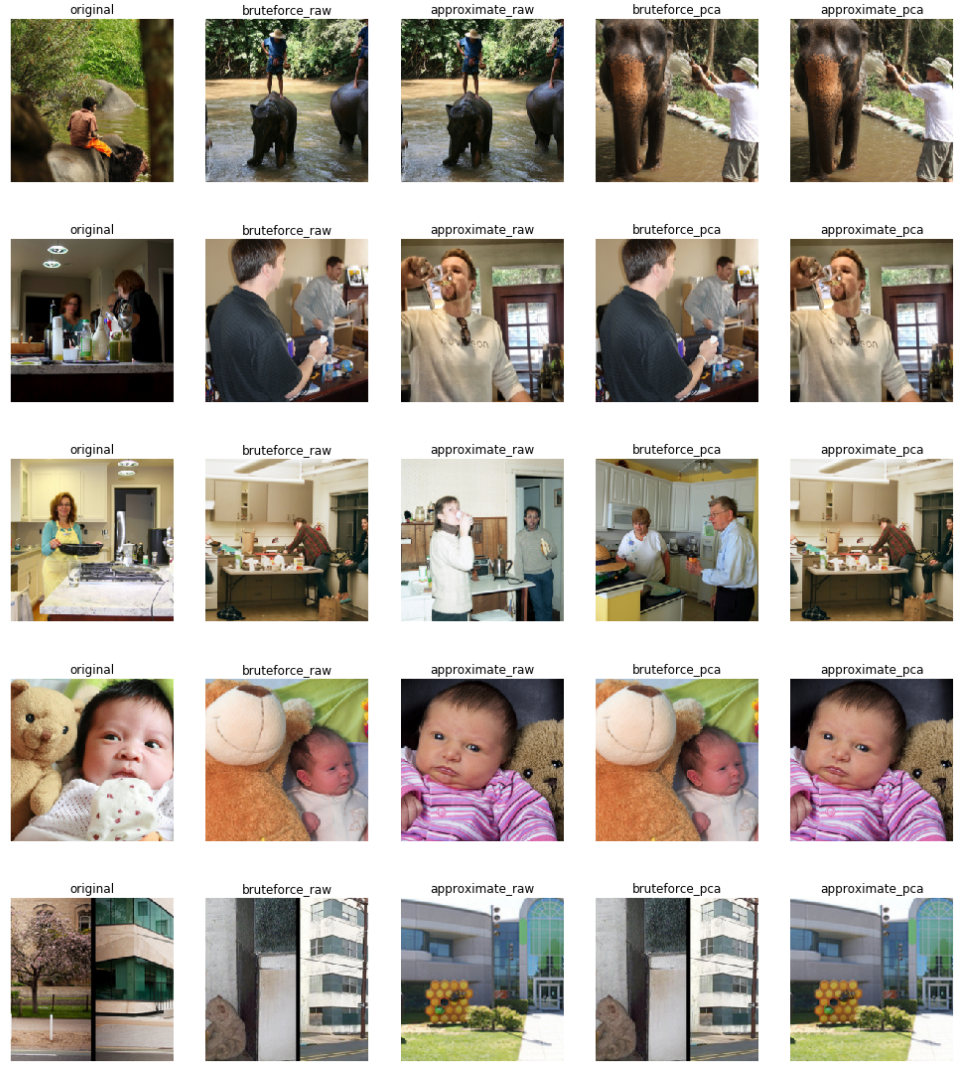
\includegraphics[width=\textwidth]{visual-faiss}
	\caption{First neighbour of some images using bruteforce and approximate faiss methods on raw and PCA features.}
	\label{fig:visual-faiss}
\end{figure}

Once again we computed the BLEU score and got very similar results. The similarity comparison with brute-force shows enough evidence to evaluate the performance of the method. \\

Finally observed that it is always a tradeoff between fast build time, fast search time and precision. When performing a single search an a whole dataset only once we would recommend using the brute-force search which is overall faster and more accurate. However when performing several search on the same dataset it could be interesting to consider a fine tuned approximate search.

\subsection{Conclusion on the results}
	To conclude on the results, we had the opportunity to compare here the performance and optimisation of 4 k-NN method. Two were computed on GPU (brute-force and Faiss) and two were computed on CPU (Annoy, NMSLIB). Our results showed that with the setup we had at hand, the GPU method: Faiss came first. For a one time usage it is most efficient to use the brute-force method proposed by Faiss. However if we need to query several time an already build index then the approximate method can bring better performance. In a CPU environment only, NMSLIB through HSNW showed some very good results and outperformed Annoy by far on our dataset. Annoy still seems to be a good solution as it still performed better than our unoptimised GPU brute-force implementation. It could also be a good choice for its simplicity.

\section{Images subgroup analysis}
	Why we do that? What difference between places365 and Imagenet. How did we proceed ? Which subgroup did we chose.
	
	\subsection{Results with places365}
	\subsection{Results with Imagenet}
	\subsection{Conclusion}
	
	which training set for our CNN for which kind of images.

\begin{thebibliography}{5}

\bibitem{large-scale-search} 
Matthijs Douze, Hervé Jégou and Jeff Johnson. 2017.
\textit{An evaluation of large-scale methods for image instance and class discovery}.

\bibitem{resnet} 
Kaiming He, Xiangyu Zhang, Shaoqing Ren, Jian Sun. 2015.
\textit{Deep Residual Learning for Image Recognition}.

\bibitem{HNSW} 
Yu. A. Malkov, D. A. Yashunin. 2017.
\textit{Efficient and robust approximate nearest neighbor search using Hierarchical Navigable Small World graphs}.

\bibitem{faiss} 
Jeff Johnson, Matthijs Douze, and Hervé Jégou. 2017.
\textit{Billion-scale similarity search with GPUs}. 

\bibitem{BLEU} 
Kishore Papineni, Salim Roukos, Todd Ward, and Wei-Jing Zhu. 2002.
\textit{BLEU: a Method for Automatic Evaluation of Machine Translation}. 


\end{thebibliography}

\end{document}